\documentclass[11pt, oneside]{article}   	% use "amsart" instead of "article" for AMSLaTeX format
\usepackage[margin=2cm]{geometry}                		% See geometry.pdf to learn the layout options. There are lots.
\geometry{letterpaper}                   		% ... or a4paper or a5paper or ... 
%\geometry{landscape}                		% Activate for for rotated page geometry
\usepackage[parfill]{parskip}    		% Activate to begin paragraphs with an empty line rather than an indent
\usepackage{graphicx}				% Use pdf, png, jpg, or eps§ with pdflatex; use eps in DVI mode
							% TeX will automatically convert eps --> pdf in pdflatex		
\usepackage{amssymb}
\usepackage{hyperref}
\usepackage{placeins}

%\date{}							% Activate to display a given date or no date



\begin{document}
\textbf{BIOL 3295 Fall 2019}

\textbf{Assignment 3 due Friday Nov 15, 1pm}
\begin{description}
\subsubsection*{Stage structure}

\item[1.] Consider a population with a projection matrix:
\[
\left[
\begin{array}{cc}
0 & 4 \\
0.9 & 0.2
\end{array}
\right]
\]
Calculate the eigenvalues. Will a population with this projection matrix increase over time?

\item[2.] The computer output gives the following:
\vspace{-3.5cm}
\begin{figure}[!ht]
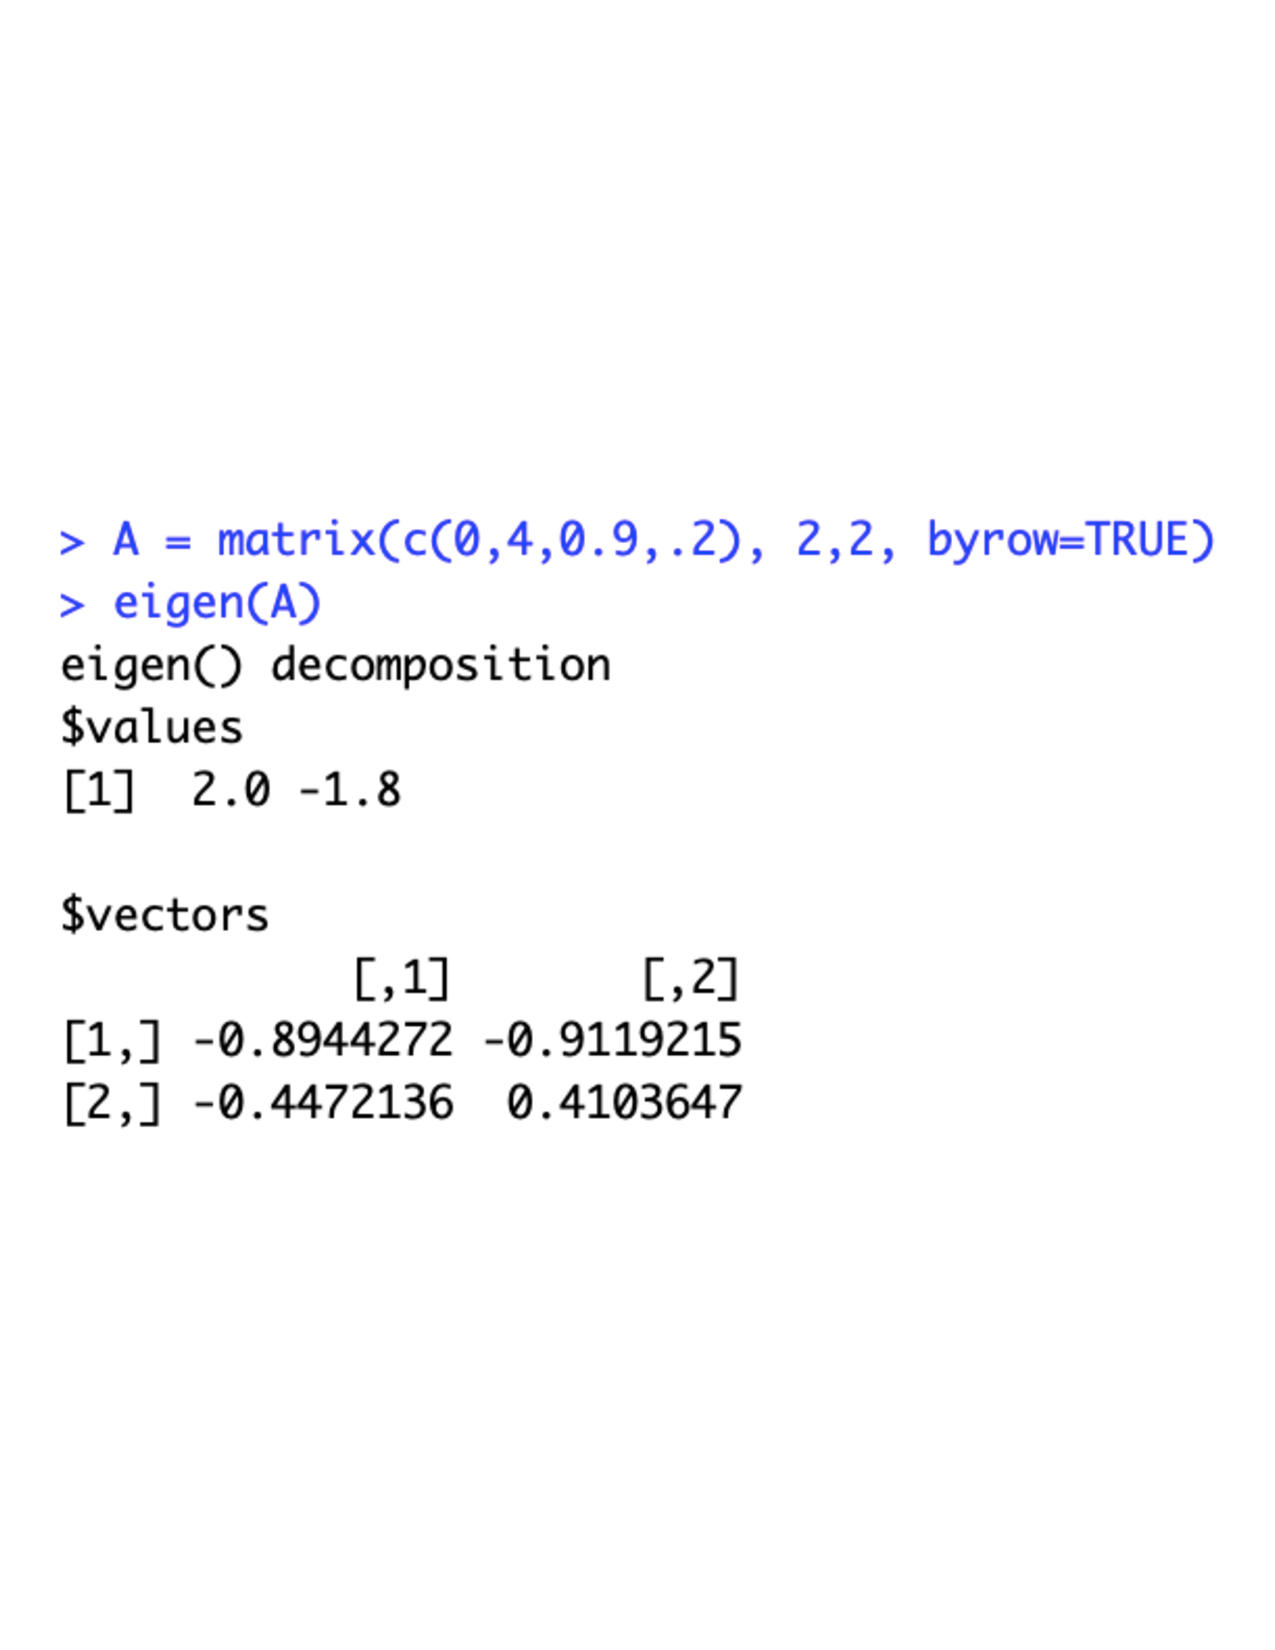
\includegraphics[height=11cm]{Routput}
\end{figure}
\vspace{-3.5cm}

 What is the eigenvector associated with the dominant eigenvalue? What will be the fraction of individuals in each stage, after a sufficiently long time?
 
 \item[3.] What are the meanings of \texttt{0} and and \texttt{0.9} in the projection matrix above? i.e., biologically, what do these numbers correspond to?
 
 \item[4.] Describe two common errors made when parameterizing matrix population models as described by \cite{Kendall}.
 
 \subsubsection*{Age at first reproduction}
  \item[5.] Consider two genotypes:\\
  \underline{Genotype 1}\\
  \[
  \begin{array}{ccccc}
  x & 1 & 2 & 3 & 4\\
  l_x & 0.5 & 0.4 & 0.3 & 0.2\\
  m_x & 0& 1 & 1& 1\\
  \end{array}
  \]

  \underline{Genotype 2} \\
  \[
  \begin{array}{ccccc}
  x & 1 & 2 & 3 & 4\\
  l_x & 0.6 & 0.5 & 0.4 & 0.3\\
  m_x & 0& 0 & 1 & 1\\
  \end{array}
\]

Calculate $R_0$ for each genotype.

\item[6.] When comparing genotypes 1 and 2, what type of trade-off is seen?
\item[7.] Give one reason why $R_0$ may be a poor measure of fitness.
\item[8.] Consult the notes \texttt{Nov\underline{ }1\underline{ }Measuring\underline{ }Fitness.pdf}. It is claimed that $m_1 = 1$ individuals per day is the maturation rate that is an evolutionarily stable strategy (ESS). Select values of $m_1$ and $m_2$ to provide further evidence that $m=1$ is the ESS (different from the example values given in the notes). Do the calculations to determine whether $m_2$ can invade.
\item[9.] If $m_1 = 1$ is an ESS, describe what must be true of $m_1$ and $m_2$ values and the calculations to determine if $m_2$ can invade. 
\end{description}

\begin{thebibliography}{10}
\bibitem[Kendall et al., 2019]{Kendall} Kendall, B. et al. 2019. Persistent problems in the construction of matrix population models.  Ecological Modelling 406: 33-43 \url{https://www-sciencedirect-com.qe2a-proxy.mun.ca/science/article/pii/S0304380019301085}
\end{thebibliography}



\end{document}  